%% ==============================
\chapter{\iflanguage{ngerman}{Methoden}{Methods}}
\label{sec:methods}
%% ==============================


\todo{laden nrrd/dicom etc.}
\todo{unsigend umrechnen / volume halbieren}
Die Implementierung dieser Arbeit orientiert sich an der Arbeit von Nguyen \cite{nguyen2012clustering}. 

Das von ihm vorgestellte Verfahren basiert auf einem zwei- beziehungsweise dreistufigen Clusteringverfahren.

Zunächst müssen die LH-Werte aller Voxel bestimmt werden. Diese drücken aus, ob ein Voxel innerhalb eines Materials oder an der Grenze zweier Materialien liegt.




Dafür müssen die Gradienten aller Voxel bestimmt werden. Wie im Paper beschrieben wurde in dieser Arbeit auch Hong's Methode \cite{hong2003method} dafür gewählt.
In diesem wird ein Approximationsbasiertes Verfahren zur Berechnung von Gradienten eines Volumens vorgestellt. 
\newline
 In Hong's Verfahren wird zur Berechnung die lokale 4x4x4 Nachbarschaft hinzugezogen. Hierbei ist zu beachten, dass der Gradient für einen Voxel nicht direkt berechnet werden kann. Der Gradient kann immer nur zwischen zwei Voxeln berechnet werden. Deshalb liegt er im Falle eines dreidimensionalen Volumens im Zentrum eins Würfels, der von 8 benachbarten Voxeln aufgepsannt wird, wie man in \autoref{fig:nachbarschaft} sehen kann. Die Knoten sind hierbei die Voxel des Volumens in denen ein Intensitätswert gespeichert ist.
\newline

\begin{figure}[!h] 
\centering 
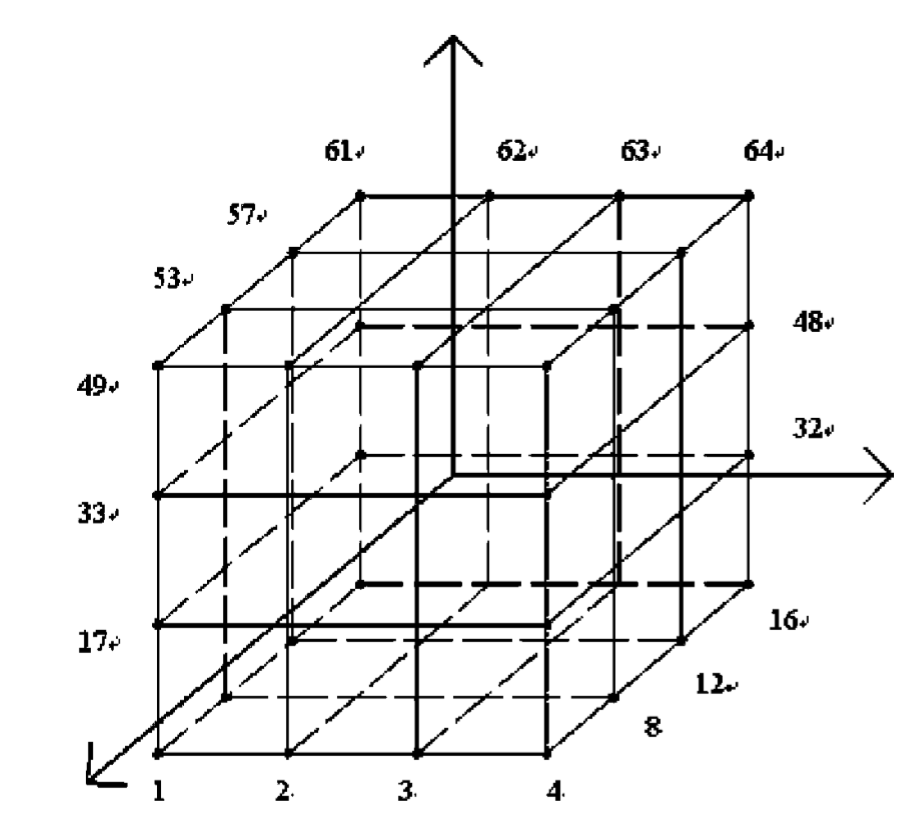
\includegraphics[width=\textwidth]{Logos/VoxelEdges.PNG}
\caption{Darstellung der lokalen 4x4x4 Nachbarschaft} 
\label{fig:nachbarschaft} 
\end{figure}
\todo{richtig bild zitieren u. evtl kleiner}




Die Funktionen für die Intensitätswerte wird im Paper mit:  $f(x,y,z) = Ax^{2}+By^{2}+Cz^{2}+2Fyz+2Gzx+2Hxy+2Ix+2Jy+2Kz+D$  approximiert. Da der Gradient die Ableitung der Intensitätsfunktion ist, erhält man den dreidimensionalen Gradientenvektor n, indem die Funktion ableitetet wird: $n = (Ax+Gz+Hy+I, By+Fz+Hx+J, Cz + Fy + Gx + K)$ .
\newline
Um den Gradienten zu Berechnen müssen die Parameter A,B,C,E,F,G,H,I,J,K  berechnet werden. Dies geschieht mithilfe der Methode der kleinsten Quadrate.

Am Ende dieses Verfahrens haben wir ein Volumen, in dem alle Gradienten gespeichert sind. Jedoch sind die Punkte um eine halbe Voxellänge verschoben. Desweiteren ist die Dimension dieses Volumens in jeder Achse um eins kleiner als das vorher gegebene Intensitätsvolumen.
Da für die Berechnung der LH-Werte jedoch der Gradient und der Intensitätswert an einer Stelle im Volumen bekannt sein muss, wurden die Intensitätwerte auf das Volumen der Gradienten umgerechenet. Dies geschah durch eine einfach Interpolation indem von allen 8 Nachbarn eines Punktes der Intensitätwert geachtelt wurde und aufaddiert. Hierbei gehen Information verloren....
\todo{abbildung für interpolation und beschreiben was verloren geht}


Zur Berechnung der Low- und High-Werte wird in Richtung der Gradienten integriert. Dazu wurde wie von Nguyen auch Heun's Methoder, eine modifizierte Euler Methode verwendet. 
\todo{quelle heuns methode}

Die hierzu benutzte Formel lauter: $u_{i+1} = u_{i} + \frac{1}{2}d(\triangledown f (u_{i}) + \triangledown f(u_{i}+d \triangledown f(u_{i}))) $
Hierbei sind $u_{i}$ und $u_{i+1}$ die Positionen des aktuellen, beziehungsweise des nächsten Voxels. $\triangledown f(x)$ beschreibt den normalisierten Gradienten für die High-Werte und den normalisierten inversen Gradient für die Low-Werte an Stelle $x$ und $d$ steht für die Schrittweite (ein Voxel).
Da das Verfahren in dieser Arbeit auf CT-Daten angewendet wird, ist das Abbruchkriterum der Integration, wenn ein Gradient mit Länge null gefunden wird. Ist dies der Fall wir der Intensitätswert dieses Voxels als Ergebnis für den Low- beziehungsweise High-Wert des Startvoxel genommen.

\todo{gewichtung erklären -> warum nicht vewendet}


Anschließend wird ein LH-Histogram über alle Werte erstellt. Die x-Achse sind hierbei die Low- und die y-Achse die High-Werte. Deren Reichweite geht von null bis zu den jeweiligen Maxima der Werte.

Auf diesem Histogram findet der erste Clusteringschritt  statt.
\todo{intensitätswert ventrikel}
Da die Intensitätswerte im Gehirn sehr nah beieinander liegen, war es nicht sinnvoll wie von Nguyen beschrieben über das komplette Histogramm mit einer Bandweite von 7\% - 9\% des maximalen LH-Wertes, das Maximum aller Low- und High-Werte, zu clustern. Das Gehirn wurde dabei als ein paar wenige, sehr große Cluster erkannt. Diese Herangehensweise mag praktibale zum Darstellen von Knochen, des kompletter Gehirns oder anderen Bereiche sein, entspricht jedoch nicht dem Ziel dieser Arbeit, das Ventrikelsystem kenntlich zu machen und zu visualisieren. Aus diesem Grund wurde die Bandbreite des Clustering auf 0,1\% des maximalen LH-Wertes gesetzt. Da so eine Bandbreite sehr Rechenaufwendig ist und bekannt ist, dass das Ventrikelsystem einen Intensitätswert um die ... hat, wurde desweiteren nur im Intensitätswertbereich von 1025 bis 1075 geclustert, um die Rechenzeiten gering zu halten. Diese Maßnahmen dienen ausschließlich dem Zweck Strukturen im Gehirn bessers unterscheiden zu können, da sie so in verschiedne LH-Cluster eingeteilt werden und damit unterscheidbar sind. Wenn das Verfahrenfür andere Zieöe genutzt werden soll, können die Parameter auf die von Nguyen vorgeschlagenen Werte gesetzt werden. 

\todo{allgemein meanschiftclustering beschreiben}



Als nächstes werden die LH-Cluster erneut mit Meanshiftclustering geclustert. Diesmal jedoch anhand ihrer räumlichen Informationen im Volumen. Im Paper von Ngujen wird hierzu kein Wert für die Bandbreite vorgeschlagen. In dieser Arbeit wird ein Wert von 10 dafür und eine minimale Distanz zu stoppen des Clusterns von 0,01 gewählt.
Nachdem alles Cluster erzeugt wurden, werden ihnen zufällige IDs von eins bis zur Anzahl an Clustern zugeteilt. Anschließend wird ein Volumen erstellt, mit den Dimensionen des ursprünglichen Intensitätsvolumens, dass nur mit nullen als Werte gefüllt ist. Warum es diese Dimension haben muss, wird später erklärt. Danach wird durch alle Cluster iteriert, und jeder Voxel in das neu erstellte Volumen an der jeweiligen Position eingetragen. Dabei ist der eingetragene Wert immer die  ID des aktuellen Clusters. Nachdem alle Cluster abgearbeitet wurden, besteht das Volumen aus ausschließlich nullen und den IDs der Cluster an den passenden Stellen.


Dieses Volumen wird als eine binäre Datei abgespeichert und in Unity geladen. Hier kann der Anwender sich entweder die Form von einzelnen IDs anschauen oder eine Reichweite von IDs. Hiermit muss er anhand der Form die Cluster erkennen, die zum Ventrikelsystem gehören, und deren IDs notieren. 

Hat er dies getan kann er im ... Programm die binäre Datei mit den IDs, die ursprüngliche Intensitätsvolumendatei laden und eine Auswahl an IDs wählen. Die ausgewählten IDs werden gemerged in das Intensitätsvolumen übernommen und erhalten dort, da der maximale Wert von CT-Daten bei ...(4400) liegt  den Wert 5000. Dieser Wert erhöht das Maximum für die Darstellung der Daten nur gering, ist dafür aber im Volumen sonst niergends enthalten. Das Ergebnis dieses Merges wird wieder als binäre Datei gespeichert.

Als letzten Schritt kann nun der Benutzer die gemerged Datei in Unity laden, und sich das Ergebnis anschauen.

\todo{letzten schritt genauer}

